\chapter{动稳定性}
\section{基础}
特征根:$\lambda=-r\pm js=-\zeta\omega_n\pm j\omega_n\sqrt{1-\zeta^2}$
$$\zeta=\frac{r}{\sqrt{r^2+s^2}}\ \ ,\ \ \omega_n=\sqrt{r^2+s^2}\ \ ,\ \ T_2=T_{1/2}=\frac{\ln(2)}{|r|}$$

Routh判据
\begin{figure}[!h]
\centering
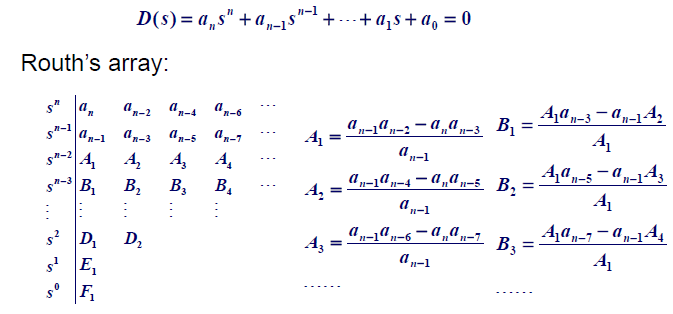
\includegraphics[width=\textwidth]{routh.png}
\end{figure}

Routh-Hurwitz判据
$$\Delta(\lambda)=a_0\lambda^4+a_1\lambda^3+a_2\lambda^2+a_3\lambda+a_4=0$$
稳定的充要条件:
$$a_0,a_1,a_2,a_3,a_4>0$$
$$R=\Delta_3=a_1a_2a_3-a_1^2a_4-a_0a_3^2>0$$

\section{纵向响应}
两对复根,大根对应短周期,小根对应长周期.

近似求解时取方程前三个高阶项求解短周期,三个低阶项求解长周期.
\subsection{短周期}
频率主要由$\Cma$决定,$|\Cma|$增加,频率增加.

阻尼主要由$\Cmq$和$C_{m\dot{\alpha}}$决定,尾容越大阻尼越大.
\begin{figure}[!h]
\centering
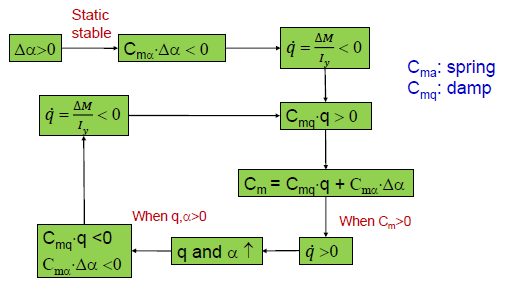
\includegraphics[width=0.8\textwidth]{sp.png}
\end{figure}

\subsection{长周期}
.
\begin{figure}[!h]
\centering
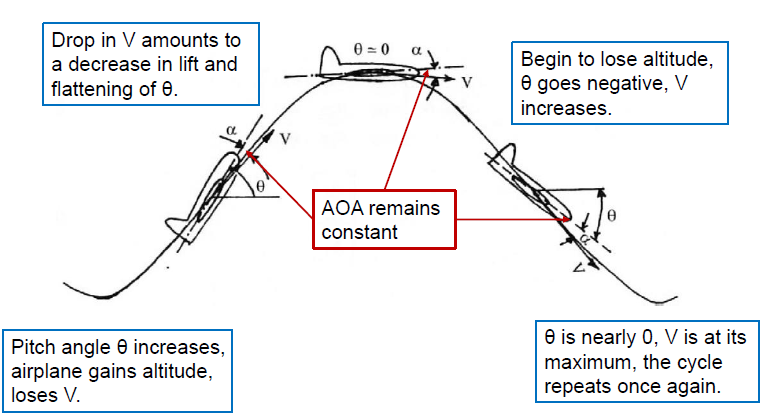
\includegraphics[width=0.8\textwidth]{ph.png}
\end{figure}

\section{横航向响应}
一个零根,两个实根,小根对应尾旋模态,大根对应滚转收敛模态,一对复根对应荷兰滚模态.
\begin{figure}[!h]
\centering
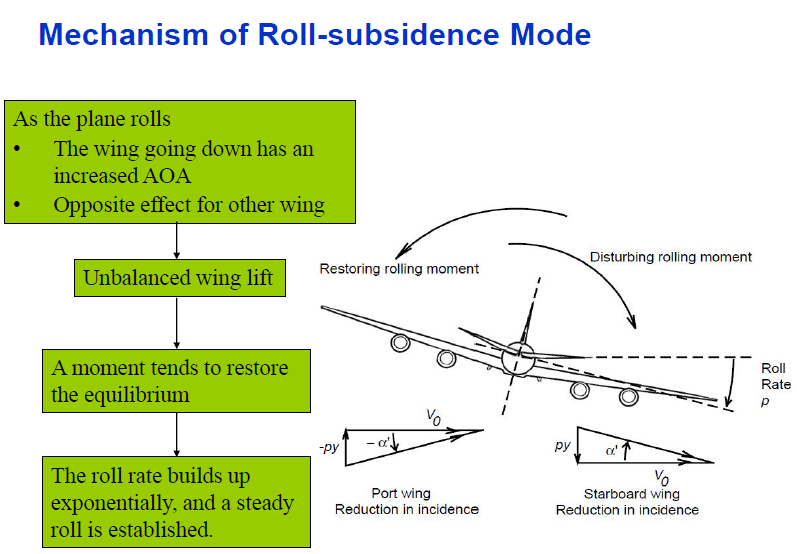
\includegraphics[width=0.8\textwidth]{rs.png}
\end{figure}
\begin{figure}[!h]
\centering
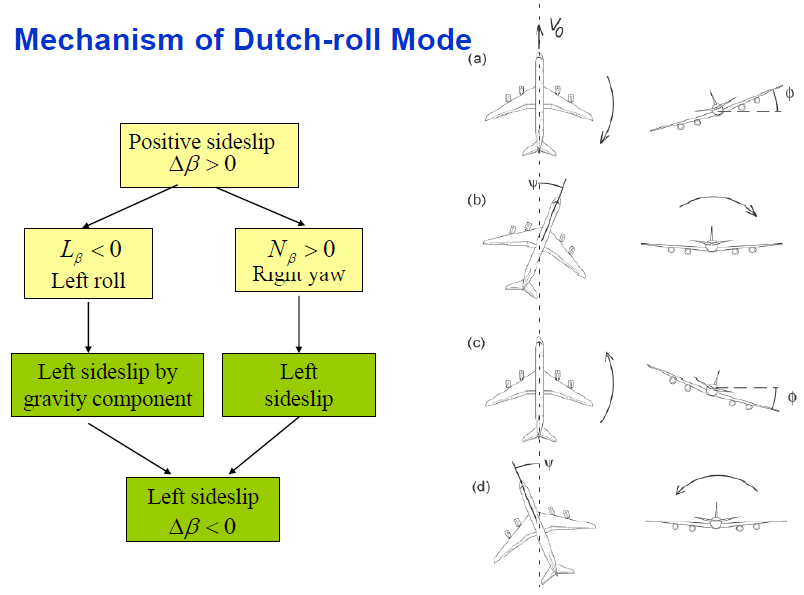
\includegraphics[width=0.8\textwidth]{dr.png}
\end{figure}
\begin{figure}[!h]
\centering
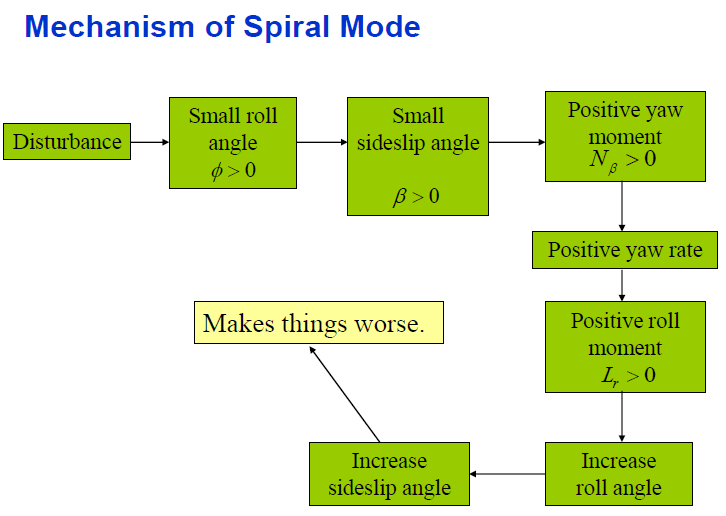
\includegraphics[width=0.8\textwidth]{s.png}
\end{figure}

\endinput